%
% fortsetzung.tex
%
% (c) 2021 Prof Dr Andreas Müller, OST Ostschweizer Fachhochschule
%
\section{Analytische Fortsetzung
\label{buch:funktionentheorie:section:fortsetzung}}
\rhead{Analytische Fortsetzung}

Wir haben schon gesehen, dass eine reelle Funktion, die in einem
Punkte eine konvergente
Potenzreihe besitzt, auf natürliche Weise auch als komplexe Funktion
betrachtet werden kann, indem man komplexe Argumente in der Potenzreihe
zulässt.
Die neue komplexe Funktion ist ein einem Kreis um den Punkt
konvergent.
Mit Hilfe der Potenzreihe kann man also immer eine Funktion auf ein
Kreisgebiet ausdehen.
Dieser Abschnitt untersucht die Frage, ob man diese Idee auch auf
noch grössere Gebiete ausdehnen kann.
\subsection{Analytische Fortsetzung mit Potenzreihen}
\begin{figure}
\centering
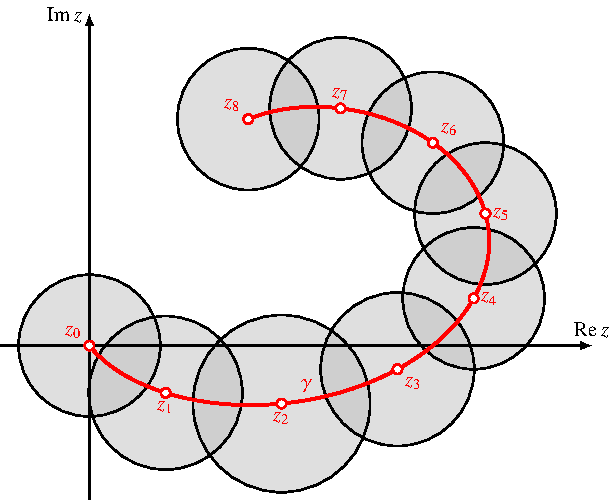
\includegraphics{chapters/080-funktionentheorie/images/forts.pdf}
\caption{Analytische Fortsetzung einer komplexen Funktion entlang einer
Kurve $\gamma$.
\label{komplex:fortsetzung}}
\end{figure}
Eine komplex differenzierbare Funktion $f(z)$ ist immer darstellbar als
Potenzreihe, und ist daher analytisch.
So kann zum Beispiel die Funktion $1/z$ als Potenzreihe um jeden
beliebigen Punkt $z_0$ entwickelt werden:
\begin{align}
f(z)
&=
\frac1z
=
\frac1{z_0-(z_0-z)}
=
\frac1{z_0}\cdot
\frac1{1-\displaystyle\frac{z_0-z\mathstrut}{z_0\mathstrut}}
=
\frac1{z_0}\sum_{k=0}^{\infty} \biggl(\frac{z_0-z\mathstrut}{z_0\mathstrut}\biggr)^k
=
\sum_{k=0}^{\infty} \frac{(-1)^k}{z_0^{k+1}} (z-z_0)^k,
\label{komplex:1durchreihe}
\end{align}
Die Koeffizienten dieser Potenzreihe sind
\[
a_k=\frac{(-1)^k}{z_0^{k+1}},
\]
und man kann den Konvergenzradius ausrechnen:
\[
\frac1{\varrho}
=
\limsup_{k\to\infty} \root{k}\of{|a_k|} = \lim_{k\to\infty}\frac1{|z_0|^{\frac{k+1}{k}}}
=
\frac1{|z_0|}.
\]
Der Konvergenzradius ist limitiert durch die Singularität bei an der Stelle
$z=0$.

Es gibt also keine einzelne Potenzreihe, die die Funktion $f(z)=\frac1z$ in der
ganzen komplexen Ebene darstellen kann.
Wählt man aber einzelne Punkte $z_0$ und $z_1$ derart, dass der Kreis
um $z_0$ mit Radius $|z_0|$ und der Kreis um $z_1$ mit Radius $|z_1|$
überlappen, dann werden die beiden Potenzreihen im Überlappungsgebiet
die gleichen Werte annehmen.

Man könnte allso eine Kurve $\gamma$ in der komplexen Ebene wählen,
entlang der man in jedem Punkt die Funktion $f(z)$ in eine Potenzreihe
entwickelt.
Liegen zwei Punkte nahe genug auf der Kurve $\gamma$, werden die
Konvergenzkreise der Potenzreihen überlappen, und die Potenzreihen
werden im Überlappungsgebiet die gleichen Werte liefern.

Selbst wenn man eine Funktion $f(z)$ nur in einem Kreis um den Punkt $z_0$
kennt, zum Beispiel durch eine Potenzreihe im Punkt $z_0$, kann man entlang
einer Kurve, die $z_0$ mit $z_1$ verbindet, in jedem Punkt eine Potenzreihe
finden, die mit der Potenzreihe in den Nachbarpunkten übereinstimmt, und
so die Definition der Funktion entlang dieser Kurve auf ein grösseres
Gebiet ausweiten, wie in Abbildung~\ref{komplex:fortsetzung} dargestellt.
Man nennt dies die {\em analytische Fortsetzung} der Funktion $f(z)$
entlange der Kurve $\gamma$.
\index{analytische Fortsetzung}
\index{Fortsetzung, analytische}

\begin{beispiel}
Wir haben bereits gesehen, dass sich die Funktion $f(z)=1/z$ in jedem
Punkt $z_0$ der komplexen Ebene in die Potenzreihe~\eqref{komplex:1durchreihe}
entwickeln lässt.
Diese Reihe lässt sich integrieren
\[
F(z,z_0)
=
\sum_{k=0}^\infty\frac{(-1)^k}{(k+1)z_0^{k+1}}z^{k+1},
\]
diese Reihe ist ebenfalls auf einem Kreis vom Radius $|z_0|$ um den
Punkt $z_0$ konvergent.
Wir vermuten natürlich, dass dies eine Darstellung des natürlichen
Logarithmus einer komplexen Zahl ist.
Natürlich ist das immer nur auf einem Kreisgebiet möglich, die Reihe
für $z=1$ ist zum Beispiel im Punkt $z=-1$ nicht konvergent.

Um eine in der ganzen komplexen Ebene definierte Funktion $\log(z)$ zu
konstruieren, müssen wir also eine analytische Fortsetzung aufbauen.
Bei der Integration haben wir eine frei wählbare Integrationskonstante
$C(z_0)$, die wir so wählen müssen, dass die Reihen im Überlappungsgebiet
übereinstimmen:
\[
F(z,z_0) + C(z_0) = F(z,z_1)  + C(z_1)
\]
für jedes $z$ im Überlappungsgebiet.
Dadurch wird aber nur die Differenz $C(z_1)-C(z_0)$ der Werte festgelegt.
Da wir Übereinstimmung mit der üblichen Definition des Logarithmus
erreichen möchten, können wir $C(1)=0$ festlegen.

\begin{figure}
\centering
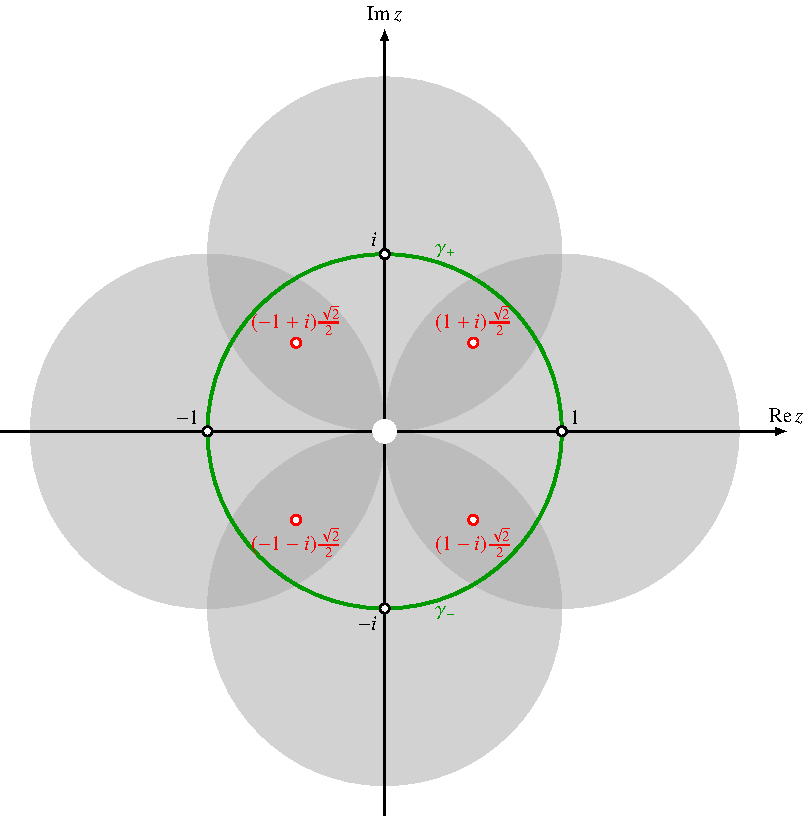
\includegraphics{chapters/080-funktionentheorie/images/fortsetzreziprok.pdf}
\caption{Analytische Fortsetzung für die Funktion $\frac1z$
entlang der Pfade $\gamma_+$ und $\gamma_-$.
\label{komplex:logfortsetzung}}
\end{figure}
Wir konstruieren jetzt die analytische Forstsetzung entlang der Kurven
$\gamma_+$ und $\gamma_-$ wie in Abbildung~\ref{komplex:logfortsetzung}
dargestellt.
Um die Differenz $C(z_1)-C(z_0)$ zu bestimmen, Werten wir die Funktionen
$F(z,z_0)$ und $F(z,z_1)$ jeweils im rot eingezeichneten Punkt aus.
Die exakte Berechnung ist etwas mühsam, da es sich ja nur um ein Beispiel
handelt, können wir die Reihen auch numerisch ausrechnen, und so die
Differenzen bestimmen:
\begin{align*}
&\text{Startpunkt $z_0=1$:}& C(1)&=0             &       &       \\
&\text{entlang $\gamma_+$:}& C(i)&= i\frac{\pi}2 & C(-1) &=  i\pi\\
&\text{entlang $\gamma_-$:}&C(-i)&=-i\frac{\pi}2 & C(-1) &= -i\pi
\end{align*}
Wir stellen fest, dass die analytische Fortsetzung der Logarthmusfunktion
entlang der Kurve $\gamma_+$ die Potenzreihe
\[
\log_+(z)
=
i\pi +\sum_{k=1}^\infty \frac{(-1)^{k+1}}{k(-1)^k}(z+1)^k
=
i\pi
-
\sum_{k=1}^\infty \frac{(z+1)^k}{k}
\]
ergibt, während man entlang der  Kurve $\gamma_-$
\[
\log_-(z)
=
-i\pi +\sum_{k=1}^\infty \frac{(-1)^{k+1}}{k(-1)^k}(z+1)^k
=
-i\pi
-
\sum_{k=1}^\infty \frac{(z+1)^k}{k}
\]
findet.
Die beiden analytischen Fortsetzungen entlang der Kurven $\gamma_+$ und
$\gamma_-$ stimmen auf der negativen reellen Achse nicht überein,
sie unterscheiden sich um $2\pi i$:
\[
\log_+(z)-\log_-(z)=2\pi i.
\qedhere
\]
\end{beispiel}

Das Beispiel zeigt, dass es im Allgmeinen eine auf der ganzen komplexen
Ebene definierte komplexe Entsprechung einer reellen Funktion nicht
zu geben braucht.
Dieses Phänomen tritt zum Beispiel auch bei der Wurzelfunktion $f(z)=\sqrt{z}$
auf.
Diese Funktion ist im Punkt $z=0$ nicht differenzierbar, man muss diesen
Punkt also aus dem Definitionsbereich ausschliessen.
Führt man man analog zum Beispiel eine analytische Fortsetzung durch,
findet man, dass sich die Werte von $f(z)$ für die beiden Wege $\gamma_+$
und $\gamma_-$ durch das Vorzeichen unterscheiden.
\subsection{Analytische Fortsetzung mit Differentialgleichungen
\label{komplex:analytische-fortsetzung-dgl}}
In Abschnitt~\ref{subsection:wegintegrale} wurde gezeigt, wie Wegintegrale
Stammfunktionen komplexer Funktionen liefern können.
Im vorangegangenen Abschnitt wurde untersucht, wie eine komplex differenzierbare
Funktion mit Hilfe von analytischer Fortsetzung entlang einer Kurve
ausgedehnt werden kann.

Sei $f(z)$ eine komplex differenzierbare Funktion.
In jedem beliebigen Punkt des Definitionsbereichs können wir $f(z)$
in eine Potenzreihe entwickeln, und natürlich auch termweise integrieren.
Es gibt also in jedem Punkt $z_0$ des Definitionsbereichs eine
Funktion $F_{z_0}(z)$, die $F'_{z_0}(z)=f(z)$ erfüllt.
Durch analytische Fortsetzung entlang einer Kurve $\gamma$ können
wir eine komplex differenzierbare Funktion $f(z)$ finden, die in einer
Umgebung der Kurve $F'(z)=f(z)$ erfüllt.

Sei andererseits $\gamma\colon[a,b]\to\mathbb C$ eine Kurve in $\mathbb C$.
Dann können wir die Werte der Stammfunktion im Punkt $\gamma(b)$ durch
\[
F(\gamma(b)) = F(\gamma(a))+\int_\gamma f(z)\,dz
\]
berechnen.

\begin{beispiel}
\begin{figure}
\centering
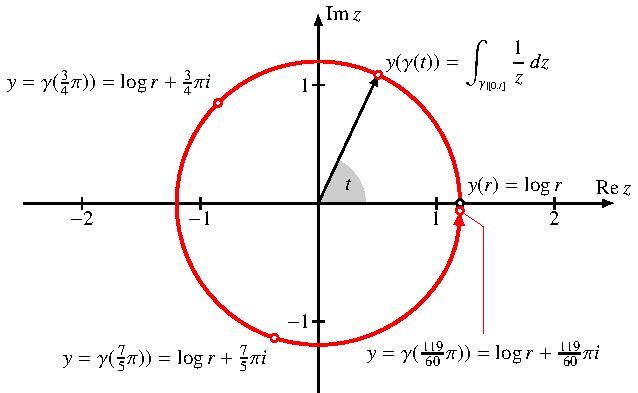
\includegraphics{chapters/080-funktionentheorie/images/logforts.pdf}
\caption{Analytische Fortsetzung des Logarithmus als Lösung der
Differentialgleichung $y'=\frac1z$.
Bei einem Umlauf um den Nullpunkt nimmt der Wert von $y(z)$ um
$2\pi i$ zu.
\label{komplex:analytische-fortsetzung-log}
}
\end{figure}
Wir bestimmen die Stammfunktion von $f(z)=1/z$.
Entlang der reellen Achse weiss man bereits, dass die Stammfunktion
der natürliche Logarithmus ist, also $F(x)=\log x$.
Um diese Stammfunktion auf $\mathbb C$ auszudehnen, verwenden wir einen
kreisförmigen Pfad von der reellen Achse bis zum Punkt $z$.
Liegt $z$ in der oberen Halbebene, wählen wir einen Pfad in der
oberen Halbebene, und umgekehrt.
Wir können die Zahl $z$ in Polarkoordinaten darstellen als $z=re^{i\varphi}$.
Ein Pfad von der reellen Achse kann mit
\[
\gamma\colon [0,1]\to\mathbb C: t\mapsto re^{it\varphi}
\]
parametrisiert werden.
Der Zuwachs der Stammfunktion entlang dieses Pfades ist
\[
F(z)-F(r)
=
\int_\gamma\frac1z\,dz
=
\int_0^1 \frac1{e^{it\varphi}}i\varphi e^{it\varphi}\,dt
=
i\varphi \int_0^1\,dt
=
i\varphi.
\]
Der Wert der Stammfunktion am Anfang der Kurve ist $\log r$, somit
folgt, dass
\[
\log z = \log r + i\varphi
\]
(Abbildung~\ref{komplex:analytische-fortsetzung-log}).
\end{beispiel}


